\documentclass{manual}


\begin{document}
	
\dominitoc[c]	
\author{par l'association {\bfseries souslebaobab}}
\title{\Huge\textbf{Manifeste du \newline \newline  {\fontsize{59}{260}\sffamily\textcolor{darkgray}{  PANAFRICANISME}}}}


\frontmatter
\maketitle



\resizebox{\textwidth}{!}{%
	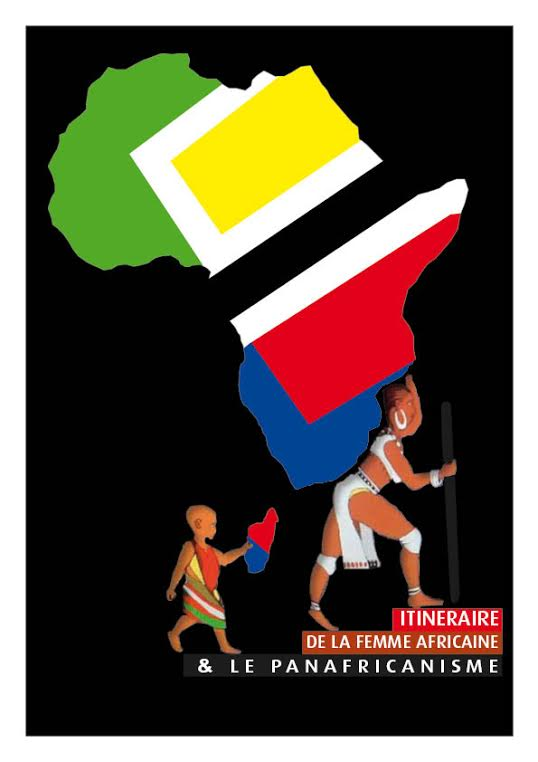
\includegraphics[scale=1.8]{cover}%	
}
\hfill \break
\vspace{300pt}
\paragraph{Deuxieme édition}
 \textcopyright Janvier 2017


Ce document, est édité sous l'initiative de l'association \textsf{Souslebaobab}.



\textit{Toute reproduction, même partielle est interdite sans le consentement de l'association.}
\hfill \break


{ Contacts de l'association:}
\begin{quote}
\begin{description}
	\item[tel]{ +33 07 68 55 84 29}
	\item[facebook 1]{ MamoushkaSouslebaobab}
	\item[facebook 2]{ Mamoushka-souslebaobab}
	\item[twitter]{ MamoushkaSouslebaobab}
	\item[youtube]{ Mamoushka Souslebaobab}
	\item[email]{ souslebaobab\_ca@yahoo.com}
	
	\item[web]{ mamoushkasoulebaobab.com/souslebaobab}
		
	\end{description}
\end{quote}



\tableofcontents
\mainmatter

	\ychapter{Panafricanisme}{
	Ce manuel, à l'usage de la jeunesse africaine se donne pour but de redonner la ferveur de nos héros aux nouvelles générations; la ferveur de Sankara, la tenacité de Lumumba, la détermination de Malcolm X, l'engagement de tous nos héros pour une meileure Afrique, libre, consciente de son histoire et préparant activement son avenir.
	
	A travers citations, biographies, faits historiques, principes sociétaux, et conseils pratiques, ce manifeste participe à l'effort d'éducation et de formation d'une génération d'espoir pour l'Afrique de demain, grande et prospère.
}

	\section{Qu'est-ce le Panafricanisme?}
	Il s'agit du mouvement intellectuel mondial dont le but est de construire, encourager et renforcer l'unité entre tous les afro-déscendants. 
	
	S'inspirant de notre destin historique commun depuis les anciens empires (Nubie, Ghana, Songhai, Egypte, Benin, Kongo,...), 
	les affres de l'esclavage, de la colonisation, des apartheids, en passant par le racisme moderne, 
	le Panafricanisme apporte une vision unique à notre futur à tous: l'UNITE.
	\ypic{nkrumah1}{Kwmamé Mkrumah, premier président du Ghana}
	Les pères des indépendances comme Kwamé Nkrumah du Ghana, Sékou Touré de Guinée, les plus modernes comme Moammar Khadafi, ou encore des afro-descendants comme Malcolm X des Etats-unis et Aimé Césaire des antilles furent parmis les fervents défenseurs de ce mouvement d'unité, primordial à notre essor.
	L'OUA, l'union africaine, est une réalisation de cet effort...

	\clearpage
	\section{Pourquoi le Panafricanisme?}
	Conscient que séparés nous n'arriverons à rien de grand dans les domaines économiques, sociaux et géopolitiques, 
	le panafricanisme promeut une synergie entre les forces sur le continent et dans la diaspora.
	
	Le constat devant une Afrique immensément riche pourtant misérablement pauvre avec une population peu éduquée, reniant sa culture,
	ignorant son histoire et en mal d'identité, reste une réalité consternante qui redonne aujourd'hui vie au panafricanisme.
	
	Conscient que séparés nous n'arriverons à rien de grand dans les domaines économiques, sociaux et géopolitiques, 
	le panafricanisme promeut une synergie entre les forces sur le continent et dans la diaspora.
	\ypic{sankara1}{Thomas Sankara, ancien chef d'état Burkinabé}
	

	Le constat devant une Afrique immensément riche pourtant misérablement pauvre avec une population peu éduquée, reniant sa culture,
	ignorant son histoire et en mal d'identité, reste une réalité consternante qui redonne aujourd'hui vie au panafricanisme.
	
	\section{Quelques célèbres panafricains?}
	\begin{itemize}
		\item Julius Nyéréré
		\item Thomas Sankara
		\item Marcus Garvey
		\item Haile Selasie
		\item W.E.B. Dubois
		\item Patrice Lumumba
		\item Check Anta Diop
		\item Malcolm X
		\item Joseph Ki Zerbo
	\end{itemize}
	\clearpage
	  \ychapter{Histoire}{
  	Description du chapitre histoire
  	
  	Prevoir le contenu en sections structurées
  } 
	% excel formula : ="\yquote{"&A2&"}{"&B2&"}{"&C2&"}{"&D2&"}"
  \ychapter{Citations}{
	Le lecteur trouvera ci-après un recueil de l'ideologie panafricaniste en quelques celèbres citations.
	
	Ces citations illustrent la pensées de beaucoup de militants et héros panafricains.
}

\yquote{Marcus Garvey}{garvey}{Si le nègre n’est pas prudent, il boira le poison de la civilisation moderne en mourra.}{L’histoire du rastafarisme commence avec Marcus Mosiah Garvey, prophète noir qui acquit une certaine popularité dans le Harlem des années 20.Né en Jamaïque en 1887, Marcus Garvey émigra aux Etats-Unis en 1916 et, l’année suivante, il fonda l’Association universelle pour l’amélioration de la condition noire (Universal Negro Improvement Association, UNIA, toujours en activité). Sous son impulsion, cette organisation devint le principal défenseur de " la rédemption par le rapatriement" (redemption trough repatriation), avec la bénédiction du Ku Klux Klan. Le Klan, en revanche, approuvait tout à fait cette purification ethnique par un départ volontaire. Très actif, Marcus Garvey créa son propre journal, The Negro World, à New York. Le slogan nationaliste de Garvey " One Aim, One God, One Destiny " en devint la devise. }
\yquote{Thomas Sankara}{sankara}{}{Thomas Sankara, 1949-1987, était un capitaine, révolutionaire marxiste, panafricaniste et chef d'état burkinabè. Sankara, que certains nomment le Ché Guévara africain était pionnier de la pensée anti- impérialiste et a lancé l'un des plus efficaces programmes de développements sur le continent africain. Sa lutte contre la corruption, son dévouement à la cause africaine au mépris de l'impérialisme lui ont valu sa vie dans un coup d'état mais son charisme et sa foi en l'afrique demeurent à jamais.}
\yquote{Maya Angelou}{angelou}{}{Maya Angelou, (1928-2014), était une poétesse, écrivaine, scénariste et activiste américaine.
	Elle est la premère femme noire a écrire un scénario de film avec le film "Georgia Georgia".
	Dans un contexte racial où la femme noire avait peu de visibilité, Maya porta haut à travers ses talents d'écriture, le flambeau de son identité et demeure aujourd'hui un exemple pour des milliers de femmes noires dans le monde. Maya a toujours milité pour les droits des afro américains, et évangélisé le panafricanisme.}

\yquote{Nelson Mandela}{mandela}{L’education est l’arme la plus puissante dont nous disposons pour changer le monde}{Nelson Mandela surnommé Madiba est un homme politique sud-africain né le 18 juillet 1918 à Mvezo et
	mort le 5 décembre 2013 à Johannesburg. Il fut président de l'Afrique du Sud entre 1994 et 1999
	En 1961 il lance l’aile armée de l’ANC dont il devient le commandant en chef et participe à une campagne de sabotage contre des installations publiques et militaires. 
	Il est arrêté en 1962 et condamné à perpétuité en juin 1964. Il reste 27 ans sur l’île de Robben où il est détenu prisonnier et devient le symbole de la lutte pour l'égalité raciale.
	Il est relâché en février 1990, à la suite de fortes pressions internationales sur le gouvernement blanc de l'Afrique du Sud (Frederik de Klerk).
	Le 30 juin 1991 l’apartheid est définitivement abolie. La même année il est élu président de l’ANC et dirige les négociations de la transition. 
	Deux ans plus tard il reçoit le prix Nobel de la paix avec le dernier président de l’apartheid (Frederik de Klerk).
	Il reste l’une des figures les plus puissantes dans l’histoire des luttes contre les inégalités et minorités en Afrique noire.}


\yquote{Kwamé Nkrumah}{nkrumah}{}{Kwamé Nkrumah (1909-1972), père de l'indépendance ghanéene, et membre fondateur de l'Union Africaine, fut un farouche combattant de la liberté de son pays, du panafricanisme et de l'anti impérialisme. Il combat virulemment le Tribalisme, une grangène contre l'essence même de l'unite panafricaine. Nkrumah mit en place le "Accelerated Development Plan for Education" un programme éducatif adapté dont l'objectif est l'émergence rapide du ghana. Apôtre du panafricanisme, Nkrumah encouragea l'étude de culture et l'histoire africaines par des cooperations avec des librairies et dénonça fermement les méthodes aliénantes de la white supremacy.}
\yquote{Um Nyobé}{nyobe}{}{Ruben Um Nyobe, surnommé Mpodol (le porte-parole1), est un dirigeant camerounais et première personnalité politique à revendiquer l'indépendance de son pays, le Cameroun, en Afrique francophone et l'unification des parties orientale (sous tutelle française) et occidentale (sous tutelle anglaise). Il est né en 1913 à Eog Makon et mort assassiné par l'armée française le 13 septembre 1958 à Libelingoï, près de Boumnyébel (actuel département du Nyong-et-Kéllé, Région du Centre)
	Il a été officiellement proclamé Héros national par l'Assemblée nationale du Cameroun le 27 juin 1991.}
\yquote{Jomo Kenyatta}{kenyatta}{}{Kenyatta a été Premier ministre du Kénya entre 1963 et 1964 puis président de 1964 à 1978. Journaliste de profession, homme politique charismatique, respectable et écouté, le Président Jomo Kenyatta était aussi un sage fort intéressé par l’Histoire du continent africain et du Kenya en particulier. Sa plus célèbre citation est, d’ailleurs, intimement liée à la colonisation de l’Afrique et aux procédés utilisés par les colonisateurs pour s’installer sur le continent africain.
	Voici donc la plus célèbre citation du Président Jomo Kenyatta :
	« Quand les missionnaires sont arrivés, nous avions les terres et eux, ils avaient la Bible. Ils nous ont appris à prier avec nos yeux fermés. Quand nous les avons ouverts, ils avaient nos terres et nous, nous avions leur Bible ».}
\yquote{Aminata Traoré}{traore}{}{Aminata Dramane Traoré est une femme politique et écrivaine malienne. L'extrait suivant d'une interview réalisée par Clarice Kamwa sur la question du retard de l'Afrique retrace bien son combat:\newline \newline
	{\itshape...Je parle rarement de retard et de rattrapage parce que si on se situe sur ce registre, on se morfond sur soi même en disant: les autres nous ont dépassé.et si nous estimons que les autres nous ont dépassé, ça veut dire , qu'il faut emprunter la voix qu'ils ont emprunté pour nous en sortir, mais il faut constater aujourd'hui que les pays les plus riches, qui prétendent nous guider, sur la voix du développement, sont confrontés aux même problèmes:A l'épineux problème de l'emploi et au problème de la paupérisation de la précarité et une bonne partie des citoyens de ces pays, qui se sont enrichis au détriment de l'Afrique veulent que leur propre pays changent de paradigme de développement.}}
\yquote{Djibo Bakary}{bakary}{}{Dirigeant syndicaliste nigérien. Membre du Parti Progressiste Nigérien, section du RDA, puis fondateur de l’Union des Forces Populaires-Sawaba. Au cours du processus menant à l’indépendance il préside le gouvernement « autonome ». Il fait campagne pour le « Non » au référendum du 28 septembre 1958 à la constitution gaulliste et représente la gauche, mais est contraint à l’exil. Il tentera un retour dans les années 1970 qui lui vaudra la prison.}
\yquote{Sékou Touré}{toure}{}{Sékou Touré (1922-1984), père de l'indépendance guinéenne et déscendant de Samoury Touré fut un militant de la décolonisation africaine. En 1956 il devient leader du Parti Démocratique Guinéen, une branche locale du Rassemblement Démocratique Africain. Farouche opposant à l'impérialisme et défenseur de la souveraineté africaine, il est l'une des figures de la fierté et du nationalisme
	panafricains. Il fut capturé par une france à laquelle il résiste toute sa vie et mourut aux USA. Sa détermination se résume en sa célèbre citation sur la liberté.}
\yquote{Malcolm X}{x}{}{Malcolm X (1925-1965), sans aucun doute, l'un des dévoués, infatiguables et charismatiques leader de l'activisme afro américain, et panafricain. Malcolm dénonça avec la plus grande fermeté la white supremacy, encouragea la création d'une nation d'afro descendante. Leader charismatique et très réaliste il fait la promotion du self defense, du self determination et contribue avec les Black Power à constituer un contre poids à l'idéologie extremement raciste de la white supremacy aux Etats-unis à son époque.
	N'étant pas un fervent pacifiste, stricte et rigoureux, Malcolm écarte de ses propres rangs ceux jugés corrompus et se sépare de la Nation of Islam. Cette détermination et cette rigueur lui firent plusieurs ennemis qui l'assassineront en 1965, lui, mais pas son idéologie.}
\yquote{Martin Luther King}{king}{}{M.L. King (1929-1968), pasteur baptiste américain, fut l'un des plus grands activistes noirs de l'histoire des états unis. Contemporain de Malcolm il pronait une lutte non violente, une désobéissance civile en accord avec les principes du chrétiens. Son action et ses idées puissantes influencent jusqu'aujourdhui le panafricanisme et la lutte pour l'unité et contre le racisme. Son célèbre discours "I have a dream" marquera à jamais les esprits et Obama lui rendit hommage en tant que premier président noir. King organisa avec succès plusieurs révoltes non violentes qui aboutirent à plus de droits.}
\yquote{Kémi Séba}{seba}{}{Kémi Séba, né Stellio Capo Chichi en 1981, est une figure du Panafricanisme moderne. Activiste, essayiste et confériencier, il est l'un des actuels fervents défénseurs de la cause noire. Son combat et sa détermination lui ont valu les foudres de l'occident.
	Il compte à son actif plusieurs livres et conférences et demeure très actif sur les réseaux sociaux, semant sans cesse les graines d'une unité panafricaine et d'une conscience identitaire}
\yquote{Farida Nabouréma}{nabourema}{}{Farida Bemba Nabouréma née en 1990 à Lomé, est une auteur et icône de l'activisme afro-déscedant contemporain. Son combat acharné contre l'oppression des régimes dictatoriaux en afrique, ses analyses perspicaces sur la situation des afro américains et ses écrits la placent au rang des jeunes engagés pour l'émergence panafricaine. "Chez l'espèce humaine, l'oppression est l'arme des prédateurs" déclare-t-elle dans ses écrits. Son essai "La pression de l'oppression" est une illustration de son travail. Elle reçoit le prix du Young African in Leadership en 2016.}
\yquote{Clarice Kamwa}{kamwa}{}{Clarice Kamwa, connue sur les réseaux sociaux sous le nom de Mamoushka, est une poètesse basée au Royaume-Uni,écrivain,humaniste, pan-africaniste et analyste politique est l'une des figures modernes du panafricanisme, la jeunesse fervente qui comprend les enjeux de notre nation, les maux auxquels nous sommes confrontés et l'urgence d'un nouvel élan d'éducation, de sensibilisation. Très active sur facebook, elle réunit "}

		  
  \ychapter{Société}{
  	Description du chapitre Société
  	
  	Prevoir le contenu en sections structurées
  }

\end{document}